\documentclass[a4paper]{article}
\usepackage{zadaci}
\usepackage[dvipsnames]{xcolor}
\usepackage{wrapfig}
\usepackage{url}
\usepackage{tikz}
\usepackage{amsmath}
\usepackage[normalem]{ulem}
\usetikzlibrary{angles,quotes}
\contestname{Studentsko natjecanje\\29. studenog 2020.}
\markright{\textbf{\textsf{Opisi algoritama}}}

\usepackage{hyperref}
\hypersetup{
    colorlinks=true,
    linkcolor=blue,
    filecolor=magenta,
    urlcolor=cyan,
}

\begin{document}

\section*{Opisi algoritama}
Zadatke, testne primjere i rješenja pripremili: Patrick Pavić, Ivan Paljak i
Krešimir Nežmah. Primjeri implementiranih rješenja dani su u priloženim
izvornim kodovima.

\subsection*{Zadatak A -- Ascii Art}
\textsf{Predložio: Ivan Paljak}\\
\textsf{Potrebno znanje: osnove programiranja, implementacija}

Ovo je u potpunosti implementacijski zadatak. Bilo je potrebno pažljivo
pročitati tekst zadatka, implementirati ono što piše u njemu piše i pokriti
sve slučajeve poput uključivanja ishodišta u sliku iako se ono ne nalazi u
najmanjem ograničavajućem okviru istaknutih točaka.

\subsection*{Zadatak B -- Brzi Biljar}
\textsf{Predložio: Krešimir Nežmah}\\
\textsf{Potrebno znanje: osnove geometrije, provjera je li točka na
pravcu}

Za $0$ odbijanja odgovor je očito uvijek $1$.

Pogledajmo prvo kako rješiti zadatak za $k = 1$. Reflektirajmo stol preko sve
četiri stranice tako da dobijemo četiri kopije stola, svaki sa svojom
reflektiranom rupom. Sada umjesto da gađamo pravu rupu s izlomljenom putanjom,
možemo zamisliti da gađamo jednu od četiriju imaginarnih rupa s potpuno
pravocrtnom putanjom.

Za veće $k$ analogno popločimo cijelu ravninu s reflektiranim kopijama stola te
tada svaka imaginarna rupa odgovara određenoj izlomljenoj putanji na pravom
stolu. Svaku kopiju stola možemo označiti uređenim parom $(x,y)$ koji označava
da na putu do tog stola u ravnini treba $x$ puta refektirati vertikalno i $y$
puta horizontalno. Originalni stol naravno ima oznaku $(0,0)$. Ako stol ima
oznaku $(x,y)$ onda je broj odbijanja na putu do pripadajuće imaginarne rupe
jednak $|x|+|y|$.

Zadatak rješavamo tako da redom od $k=0$ do $k=n$ prođemo po svim parovima
$(x,y)$ za koje je $x+y=k$ (kojih ima $\mathcal{O}(k)$) te uračunamo putanju za
taj stol. Potrebno je paziti da se na tom pravcu nije dosad našla već neka
druga rupa ili neki od vrhova stola. Zato je potrebno pamtiti koeficijente
smjera već obiđenih pravaca u nekoj strukturi (npr.\ \texttt{std::set}) kako bi
provjerili postoji li već taj pravac od prije. Nakon obrađivanja stolova za
određeni $k$, u strukturu dodajemo nove pravce. Koeficijente smjera pravaca
najlakše je pamtiti kao par cijelih brojeva koji predstavlja do kraja skraćen
razlomak. Ukupni broj obiđenih stolova je $\mathcal{O}(n^2)$ pa je ukupna
složenost $\mathcal{O}(n^2 \log n)$.

\subsection*{Zadatak C -- Carska Civilizacija}
\textsf{Predložio: Krešimir Nežmah}\\
\textsf{Potrebno znanje: dinamičko programiranje, optimizacije prijelaza}

Ako je udaljenost dvije uzastopne izabrane postaje jednaka $d$, označimo s
$f(d)$ ukupno zadovoljstvo svih stanovnika s tom vožnjom duljine $d$, tj. $f(d)
= |d-d_1|+\ldots+|d-d_n|$.  Umjesto da sumiramo zadovoljstvo po stanovnicima,
lakše je promatrati ukupno zadovoljstvo kao sumu od $f(d)$ po svim vožnjama.

To dovodi do rješenja dinamičkim programiranjem. Neka $dp[i]$ označava najveće
zadovoljstvo ako moramo uzeti postaju broj $1$ i broj $i$ te neke između njih.
Stanja ima $n$, a prijelaz računamo u $\mathcal{O}(n)$ tako što biramo preko
koje postaje ćemo napraviti vožnju sa $i$.  Prijelaz je moguće ubrzati
koristeći svojstva funkcije $f$. Naime, kako je $f$ nastala sumiranjem
apsolutnih vrijednosti (koje su konveksne funkcije), onda je i funkcija $f$
konveksna.

Recimo da smo u dinamici trenutno na poziciji $i$ te da promatramo dva
potencijalna prijelaza na pozicijama $a$ i $b$ $(a < b)$. Prijelaz preko $a$
donosi $dp[a] + f(x_i - x_a)$, a preko $b$ donosi $dp[b] + f(x_i - x_b)$. Zbog
konveksnosti, razlika $(dp[a] - dp[b]) + f(x_i - x_a) - f(x_i - x_b)$ s obzirom
na fiksne $a$ i $b$ u odnosu na $i$ je rastuća. To znači da binarnim
pretraživanjem možemo pronaći indeks $i$ za koji će prijelaz $a$
\textit{prestići} prijelaz $b$. Ključno je uočiti da nakon tog trenutka
prijelaz $b$ više nikad ne može biti optimalan pa ga ne trebamo više
promatrati.

Prilikom obilaska stanja u povezanoj listi potrebno je pamtiti skup prijelaza
kandidata koji bi u nekom trenutku mogli postati optimalan prijelaz. U svakom
trenutku vrijedit će da su ti prijelazi sortirani po veličini, stoga je optimum
uvijek na krajnjem desnom kraju. Za svaka dva susjedna prijelaza binarnim
pretraživanjem odredimo trenutak u kojem će jedan prestići drugog. Ta
prestizanja promatramo kao događaje koje pamtimo u globalnoj strukturi i
izvršavamo u odgovarajućem trenutku. Na taj način jedino što preostaje je
podržati brisanje iz takve strukture. Prilikom brisanja, prethodnik i
sljedbenik izbrisanog prijelaza postat će susjedni pa sada za njih računamo
trenutak prestizanja. Dodavanjem u strukturu nakon obrađivanja svakog stanja
nastaje novi par za prestizanje pa se to rješava analogno brisanju.

Funkciju $f$ moguće je unaprijed izračunati u složenosti $\mathcal{O}(m \log m
+ maxd)$ ili u složenosti $\mathcal{O}(\log m)$ po pozivu uz prethodno
sortirani niz $d$-ova.

Ukupna složenost je $\mathcal{O}(n \log^2 n)$ ili $\mathcal{O}(n \log n * maxd)$.

\subsection*{Zadatak D -- Drugi Dio}
\textsf{Predložio: Patrick Pavić}\\
\textsf{Potrebno znanje: osnove geometrije}

Neka točke $A$ i $B$ tvore optimalno rješenje. Neka je kut između dužine $\overline{AB}$ i
pravca paralelnog s $x$ osi označen s $\phi$. Sada početni izraz možemo raspisati na
sljedeći način ako uzmemo da je $D$ euklidska udaljenost tih točaka:

  \[\frac{D \sin \phi + D \cos \phi}{D} = \sin \phi + \cos \phi\]


Taj izraz se minimizira kada je $\phi$ što bliže $0$ il $90$ stupnjeva. Promatrat
ćemo dva slučaja, najbliže $0$ stupnjeva i najbliže $90$ stupnjeva. Slučajevi su
analogni stoga promatrajmo slučaj $90$ stupnjeva. Pogledajmo sljedeći crtež.

\begin{figure}[h]
  \centering
  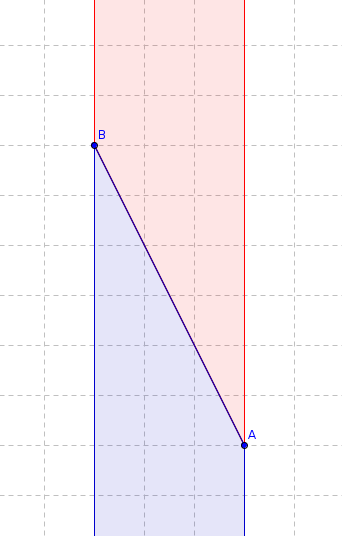
\includegraphics[height=6cm]{pic/D_edit.png}
\end{figure}


Budući da se radi o optimalnom rješenju, u crvenom se području ne smije
nalaziti točka jer bi ona zatvarala veći kut s točkom $A$, odnosno u plavom
području s točkom $B$. Iz toga slijedi da kada sortiramo točke po
$x$-koordinati one se nalaze na susjednim mjestima. Preostaje samo provjeriti
sve susjedne parove. U drugom slučaju sve vrijedi analogno, jedino sortiramo po
$y$-koordinati.

\subsection*{Zadatak E -- Ekstremna Ekspedicija}
\textsf{Predložio: Patrick Pavić}\\
\textsf{Potrebno znanje: vjerojatnosti, očekivanja, rad sa stablima, LCA}

Promatrajmo put između čvorova $A$ i $B$. Označimo čvorove na tom putu redom $A
= v_1, v_2, \ldots , v_k = B$.  Neka $E[U;V]$ označava očekivanu duljinu puta
između tih dvaju čvorova. Zato što se radi o stablu vrijedi sljedeće:

\[E[A;B] = E[v_1;v_2] + E[v_2;v_3] + \ldots + E[v_{k-1};v_k]\]

Sada preostaje samo izračunati $E[a_i;b_i]$ odnosno $E[b_i;a_i]$ za svaki brid
te pozbrajati redom. To zbrajanje može se izvršiti pomoću LCA algoritma i
prefiks suma u $\mathcal{O}(\log N)$ po upitu uz $\mathcal{O}(n \log n)$
predizračun.

Zamislimo neki brid $(u, v)$. Trenutno se nalazimo u čvoru $u$ te želimo
napraviti korak do čvora $v$. Neka $deg(u)$ označava stupanj tog čvora. Postoji
vjerojatnost $\frac{(deg(u) - 1)}{deg(u)}$ da ćemo otići u komponentu s čvorom
$u$ maknemo li brid $(u, v)$. Zanima nas očekivano vrijeme prije nego što
ponovno dođemo u čvor $u$. Prema stacionarnoj distribuciji u Markovljevim
lancima, to je $\frac{D}{(deg(u) - 1)}$ gdje je $D$ suma svih stupnjeva čvorova
u tom grafu, tj. u ovom slučaju toj komponenti. To vrijeme ćemo nazvati
$E[vraćanja]$. Tada dobivamo sljedeći izraz:

\[E[u;v] = \frac{deg(u) - 1}{deg(u)}(E[vraćanja] + E[u;v]) + \frac{1}{deg(u)}\]
\[deg(u)E[u;v] = (deg(u) - 1)E[vraćanja] + (deg(u) - 1) E[u;v] + 1\]
\[E[u;v] = \frac{D(deg(u) - 1)}{deg(u) - 1} + 1\]
\[E[u;v] = D + 1\]

Iz toga slijedi da je očekivano vrijeme da prijeđemo iz čvora $u$ u susjedni
čvor $v$ zapravo zbroj svih stupnjeva čvorova u komponenti koja sadrži čvor u
koju dobijemo kada maknemo taj brid.  Sada je lagano odgovoriti na upite.

\subsection*{Zadatak F -- Fenomenalni Fenjer}
\textsf{Predložio: Ivan Paljak}\\
\textsf{Potrebno znanje: Osnove geometrije, \textit{sweep-line} algoritam}

Primijetimo najprije da možemo ignorirati sve točke čija je $y$-koordinata po
apsolutnoj vrijedonsti strogo veća od radijusa kružnice $r$.

Zamislimo da guramo zadanu kružnicu po $x$-osi slijeva nadesno te primijetimo
da će se svaka točka najprije biti desno od kružnice, potom će \textit{udariti}
u desni dio kružnice, pa će se nalaziti unutar kružnice sve dok ne
\textit{udari} u njen lijevi rub i nakon toga zauvijek izađe iz kružnice.
Promatrajmo za svaku točku (kuću) sve moguće vrijedonst $x$-osi središta
kružnice (fenjera) dok se ta točka nalazi na rubu ili u unutrašnjosti kružnice.
Primijetit ćemo da te vrijednosti čine \textit{interval} na $x-osi$.

Ako za svaku točku izračunamo o kojem se intervalu radi, zadatak smo sveli na
sljedeći problem: zadano je $n$ intervala na $x$-osi, odredi najveći broj
intervala koji sadrže neku zajedničku točku. Ovaj problem jednostavno možemo
riješiti koristeći \textit{sweep-line} algoritam. Odnosno, prolazit ćemo po
krajnjim točkama intervala slijeva nadesno i putem pamtiti trenutni broj
otvorenih intervala. Kada detektiramo početak nekog intervala, broj otvorenih
intervala porast će za $1$, a u protivnom će se smanjiti za $1$. Najveći broj
otvorenih intervala kojeg zateknemo u nekom trenutku našeg algoritma predstavlja
rješenje zadatka.

Vremenska složenost je $\mathcal{O}(n \log n)$,

\subsection*{Zadatak G -- Gospodar Gljiva}
\textsf{Predložio: Patrick Pavić}\\
\textsf{Potrebno znanje: napredna kombinatorika}

Rješenje zadtatka je ${mn \choose n} \cdot \frac{1}{n(m - 1) + 1}$. Takve
skupove brojeva možemo promatrati kao stabla spojimo li svaki čvor $x$ s čvorom
$\lfloor\frac{x - 1}{k}\rfloor$. Tada zapravo brojimo nešto što se zove \textit{k-ary tree}, tj.
poopćenje binarnih stabla. U slučaju za $k = 2$ rješenje je zapravo $n$-ti
Catalanov broj, a općenito rješenje je tzv. \textit{Fuss Catalan} broj. Više o tome na
sljedećoj \href{https://en.wikipedia.org/wiki/Fuss%E2%80%93Catalan_number}{poveznici}.

\subsection*{Zadatak H -- Hvalevrijedan Hitac}
\textsf{Predložio: Ivan Paljak}\\
\textsf{Potrebno znanje: DFS obilazak stabla, pophlepni algoritmi}

Rješenje postoji ako i samo ako je broj zelenih meta neparan.

Pokažimo prvo da rješenje ne postoji ako je broj zelenih meta paran. Dokaz je
induktivan. Ako nema zelenih meta, očito je nemoguće. Inače, biranjem bilo koje
zelene mete, stablo se raspada na više komponenti (ne brojeći originalni čvor)
koje u zbroju imaju neparan broj zelenih meta. To je moguće samo ako barem
jedna od komponenti ima neparno mnogo zelenih meti. Nakon promjene boje u toj
komponenti, ona će imati parno mnogo zelenih meta pa induktivno neće postojati
rješenje za tu komponentu.

Analogno induktivno razmišljanje za neparni broj meta pokazuje da je potrebno
pronaći metu takvu da sve preostale komponente imaju paran broj zelenih meta.
Jedan način za napraviti validan izbor je ukorijeniti stablo u bilo kojem čvoru
te uvijek odabirati najdublju zelenu metu. Dubine svakog čvora moguće je
odrediti dfs obilaskom stabla, a pronalaženje najdubljeg čvora u svakom
trenutku moguće je koristeći prioritetni red. Nakon biranja čvora potrebno ga je
označiti kao obrađenog, promijeniti boju susjedima te ih potencijalno ih ubaciti u
prioritetni red.

Ukupna složenost je $\mathcal{O}(n \log n)$.

\subsection*{Zadatak I -- Izvanredna Isplata}
\textsf{Predložio: Krešimir Nežmah}\\
\textsf{Potrebno znanje: osnovno dinamičko programiranje, ograničavanje odgovora}

Neka $opt(x)$ i $grd(x)$ označavaju redom koliko je najmanje kovanica potrebno
da bi se isplatio iznos $x$ te koliko bi kovanica potrošio pohlepni algoritam.
Sustav kovanica nije izvanredan ako i samo ako postoji protuprimjer, tj.
prirodni broj $k$ takav da je $opt(k) \ne grd(k)$.

Označimo s $k$ najmanji takav protuprimjer. Ključna zamjedba je da takav
protuprimjer ne može biti prevelik, ograničen je sa $2 \cdot c_n$.

\textit{Dokaz}

Ako je $k$ najmanji protuprimjer, to je najmanji broj za koji postoji $c_i$
takav da je $grd(k) \ne grd(k - c_i) + 1$. Kada bi vrijedilo $k \ge c_n$ i $k -
c_i \ge cn$, onda bi također vrijedilo $grd(k - c_n) \ne grd(k - c_i - c_n) +
1$, što je u kontradikciji s minimalnošću od $k$. Dakle, mora vrijediti $k -
c_i < c_n$, pa je $k < 2 \cdot c_n$.

Preostaje provjeriti poklapaju li se vrijednosti od $opt(x)$ i $grd(x)$ za
prvih $2 \cdot c_n$ prirodnih brojeva, što se može napraviti jednostavnom
primjenom dinamičkog programiranja u složenosti $\mathcal{O}(n \cdot c_n)$.

\clearpage

\subsection*{Zadatak J -- Jači Jovsi}
\textsf{Predložio: Patrick Pavić}\\
\textsf{Potrebno znanje: olbat stablo, dinamičko programiranje}

Izgradimo \textit{olbat stablo} (\textit{palindromsko stablo}, \textit{eertree})
nad nizom znakova. Sada ćemo dinamičkim programiranjen izračunati odgovor za
svaki čvor (tj.\ palindrom) te ga pomnožiti s brojem pojavljivanja u nizu.
Za svaki čvor $X$ postoji čvor $BK$ -- najveći palindrom koji je sufiks
palindroma $X$ te $PAR$ što je palindrom koji nastaje micanjem prvog i zadnjeg
znaka iz tog palindroma. U olbat stablu to su čvor u koji pokazuje backedge i
čvor koji je roditelj tog čvora, zato oznake $BK$ i $PAR$. Stanje dinamike će
se sastojati od oznake između $0$ i $2$ te čvora $X$.

Oznaka $1$: rješenje kad bismo u prvom potezu ostavili baš taj palindrom\\
Oznaka $0$: kada bismo ostavili ili taj palindrom ili bilo koji palindrom koji je prefiks početnog.\\
Oznaka $2$: kada bismo u prvom potezu ostavili ili taj palindorm ili bilo koji podpalindorm.\\

Podpalindrom palindroma $X$ je svaki palindrom koji se nalazi kao podriječ unutar $X$.

Prijelazi dinamike su:
\begin{align*}
  dp(X, 1) &= dp(PAR, 2) + 1 \\
  dp(X, 0) &= dp(BK, 0) + dp(X, 1) \\
  dp(X, 2) &= dp(PAR, 2) + dp(X, 1) + 2 \cdot dp(BK, 0)
\end{align*}

Završni odgovor za čvor $X$ spremljen je u $dp(X,1)$.

Vremenska složenost je $\mathcal{O}(n)$.

\subsection*{Zadatak K -- Klasična Karantena}
\textsf{Predložio: Ivan Paljak}\\
\textsf{Potrebno znanje: sortiranje, pohlepni algoritmi}

Razmatrat ćemo slučaj u kojem pokušavamo maksimizirati broj ljudi s maskama
u birtiji. Minimizacija broja maski je analogna.

Pretpostavimo da smo pronašli neki optimalan poredak ljudi $a_1$, $a_2$, \ldots,
$a_n$ koji maksimizira broj maski u birtiji. Promatrajmo kako izgleda niz
$p_{a_1}$, $p_{a_2}$, \ldots, $p_{a_n}$. Preciznije, promatrat ćemo neka dva
susjedna elementa $a_i$ i $a_{i+1}$ za koje vrijedi $p_{a_i} > p_{a_{i+1}}$.
Primijetimo da kada bismo tim elementima zamijenili mjesta, broj ljudi s
maskama u birtiji mogao bi samo narasti. Stoga zaključujemo da poredak ljudi
uzlazno sortiran po vrijednostima $p_i$ također rezultira maksimalnim brojem
ljudi s maskama.

\end{document}
%%% Local Variables:
%%% mode: latex
%%% mode: flyspell
%%% ispell-local-dictionary: "croatian"
%%% End:
